\chapter{Marco teórico}
En esta sección entramos en detalle el marco conceptual y el marco tecnológico. En la primera sección se verá la forma de aprovechar los videojuegos para la enseñanza, sus ventajas y la forma de enseñanza que comúnmente aprovechamos con estos, además tocamos temas relacionados a la programación por bloques y la metodología de software a usar y sus artefactos. En la segunda sección discutimos de tecnologías aptas para la realización del proyecto.

\subsection{Marco Conceptual}
\subsubsection{Game-based learning y educación colaborativa}
Game-based learning es “en formación en la cual los contenidos teóricos son presentados por medio de un videojuego” \cite{gamelearn2014a} y contienen elementos como \cite{gamelearn2017a}:
\begin{itemize}
    \item Historia para darle inmersión a los jugadores
    \item Gamificación, como rankings o un sistema de puntos
    \item Feedback inmediato, algunos juegos tienen información como en que se equivocaron y una oportunidad de realizarlo otra vez
    \item Simulación de una situación de la vida real, permitiendo la práctica segura en ambientes cercanos a donde aplicarán su conocimiento
\end{itemize}

Los videojuegos pueden ser una muy poderosa herramienta para el aprendizaje: permiten el aprendizaje \textit{Just In Time} que bajo desafíos realizables empujan al 
jugador a ser competente y nos ayudan a fomentar el pensamiento crítico \cite{levasseur-a}. 
El aprendizaje \textit{Just In Time} ofrece el conocimiento necesario para hacer una tarea justo cuando es necesario \cite{unknown2017a}. 
Hay métodos en los que la enseñanza \textit{JIT} ocurre naturalmente como ver un video de \textit{Youtube} cuando no sabemos cómo realizar una tarea, 
en los videojuegos es natural cuando hay introducciones a acciones en el juego como la forma en la que lo invocamos o las acciones que realizan, 
ya sea mostrando una interfaz gráfica con la forma de invocarlo.
Se encontró que los estudiantes en el aprendizaje colaborativo los alumnos se enseñan uno al otro al responder a dudas y 
clarificar preconcepciones, desarrollan comunicación oral y capacidad de liderazgo, aumenta la retención del material, 
la responsabilidad y expone a los alumnos a perspectivas diversas \cite{university-a}.
Se ha encontrado que los videojuegos colaborativos agregan ventajas como el trabajo en equipo, el pensamiento creativo, 
la comunicación y la colaboración \cite{romano-a}.

\subsubsection{Block-based programming}
Block-based programming se ha establecido como la forma de introducir a aquellos que quieren aprender a 
programar seguido por el éxito de Scratch y Code.org \cite{block_based_programming}. 
Este método de programación usa piezas de un rompecabezas como metáfora para proveer al usuario pistas sobre cuales instrucciones son válidas \cite{block_based_programming}. 

\subsubsection{Kanban}
Kanban es una metodología ágil para el desarrollo de software con un énfasis 
en la entrega continúa teniendo en cuenta la capacidad del equipo \cite{romano-a}. 
Las métricas de Kanban son las siguientes \cite{najera2018a}:
\begin{itemize}
    \item \textbf{Diagrama de flujo acumulativo \ref{fig:flujo_acumulativo}:} Provee información relacionada con la capacidad del equipo. Está basado en tiempo y muestra cómo se mueven las tarjetas de izquierda a derecha en el tablero. La altura de las bandas muestra el número de tarjetas en esa etapa durante cierta unidad de tiempo.
    \begin{figure}[h]
        \caption{Diagrama de flujo acumulativo}
        \centering
        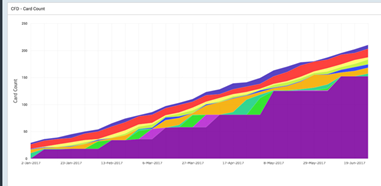
\includegraphics[width=0.5\textwidth]{flujo_acumulativo.png}
        \label{fig:flujo_acumulativo}
    \end{figure}
    \item \textbf{Gráfica de distribución de tiempos de ciclo \ref{fig:distribucion_tiempos_ciclos}:} Es útil para ver la frecuencia con la que las tarjetas son completadas a lo largo del tiempo.
    \begin{figure}[h]
        \caption{Gráfica de distribución de tiempos de ciclo}
        \centering
        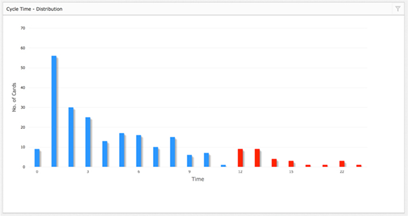
\includegraphics{distribucion_tiempos_ciclos}
    \end{figure}
\end{itemize}

\subsection{Marco tecnológico}
Para el desarrollo de este proyecto es necesario tener herramientas para las partidas con otros usuarios, así como manera de usar librerías probadas y comúnmente usadas.

\subsubsection{Unity3D}
Es un motor que permite diseñar videojuegos. Permite usar C# para programar el juego, compilando, usando Mono. \cite{unity2019} Es un motor muy capaz que permite desarrollar videojuegos 2D y 3D, con una variedad de herramientas para facilitar el desarrollo.
Unity puede crear el juego para varios entornos, como consolas de videojuegos como la Nintento Switch, el Xbox One, PS4, Windows, MacOS, Linux, Android, iOS, o la web mediante WebGL [24]. La ventaja del entorno web es la posibilidad de conectar Unity con la pagina web que lo alberga, con esto puede puedo interactuar con elementos HTML o con librerías JS, en este caso lo conectaremos con Blocky.
\begin{figure}
    \caption{Algunas capacidades de Unity para el desarrollo de videojuegos: animaciones, máquina de estados y para videojuegos 2D, un editor de sprites}
    \centering
    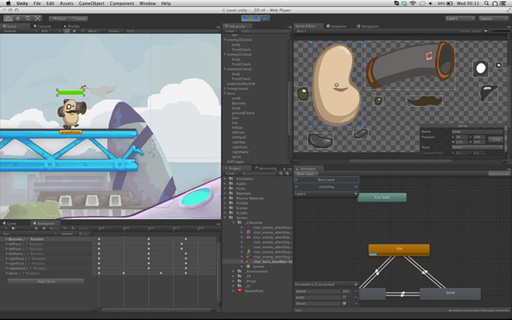
\includegraphics{unity}
\end{figure}

\subsubsection{Blocky}
Librería de Google que permite al usuario escribir código usando bloques como se nota en la \ref{fig:blocky_example} y compila el resultado a diferentes lenguajes entre ellos Javascript, Dart, Python, Lua y PHP.

\begin{figure}
    \caption{Un ejemplo de un juego usando la librería de Blocky}
    \centering
    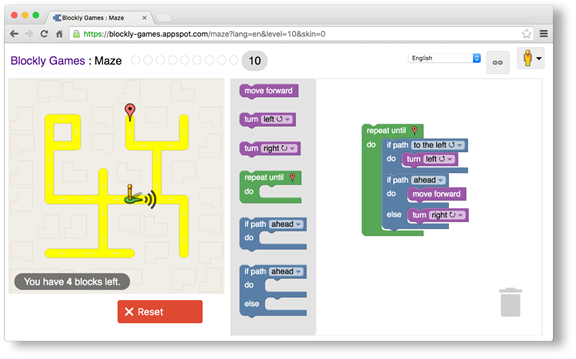
\includegraphics{blocky_example}
    \label{fig:blocky_example}
\end{figure}

\subsubsection{ASP .NET Core}
Framework para sitios web de Microsoft. Será usado como la base para hospedar la API del servidor, servir los archivos del juego, así como páginas de landing y de creación de lobbies.

\subsubsection{SignalR}
Es una librería de Microsoft que nos permite hacer comunicación en tiempo real web. Permite ser usado para crear RPC, o llamadas de procedimiento remoto. Su principal ventaja es que mandar mensajes al servidor es muy fácil a otras soluciones, hay una API definida que la librería se encarga que de que en cada request sea cumplida el schema de la API y se encarga de la serialización y deserialización de cada comunicación. Así como pasar información de cambios al cliente ocurre de manera rápida, maneja el protocolo de transferencia y evita mucha configuración que de otra forma seria necesario.

\subsubsection{Git}
Git es el sistema de control de versiones más popular del mundo, fue creado en 2005 por Linus Torvalds [27]. Es un ejemplo de un DVCS, un sistema distribuido de control de versiones, a diferencia de sistemas donde en un solo lugar esta todo el historial de versiones como CVS o Subversion, en Git todas las copias funcionales de código son un repositorio que contiene todo el historial de versiones.
En comparación con otros sistemas, Git está diseñado para que la creación de ramas y tags sean operaciones baratas, por lo tanto, rápidas.

Github es un servicio de hospedaje de repositorios Git \cite{finley2012a}. Se uso como \textit{repositorio remoto} para sincronizar cambios, además de aprovechar sus funciones para crear pipelines para el continous deployment.